\begin{section}{Results}
In this section, we briefly introduce some implementation details and present results by our extended neural style transfer methods. Furthermore, we also show the results of fusing different neural style transfer methods, which combine different style losses. In the following, we refer the four extended style transfer methods introduced in Sec.~\ref{sec:methods} as \emph{linear}, \emph{poly}, \emph{Gaussian} and \emph{BN}, respectively. The images in the experiments are collected from the public implementations of neural style transfer\footnote{{\label{fn:mxnet-neural}{https://github.com/dmlc/mxnet/tree/master/example/neural-style}}}\footnote{{{https://github.com/jcjohnson/neural-style}}}\footnote{{{https://github.com/jcjohnson/fast-neural-style}}}. 



\begin{paragraph}{Implementation Details}
In the implementation, we use the VGG-19 network~\cite{vgg} following the choice in~\cite{neuralart}. We also adopt the \emph{relu4\_2} layer for the content loss, and \emph{relu1\_1}, \emph{relu2\_1}, \emph{relu3\_1}, \emph{relu4\_1}, \emph{relu5\_1} for the style loss. The default weight factor $w_l$ is set as 1.0 if it is not specified. The target image $\mathbf{x}^*$ is initialized randomly and optimized iteratively until the relative change between successive iterations is under 0.5\%. The maximum number of iterations is set as 1000. For the method with Gaussian kernel MMD, the kernel bandwidth $\sigma^2$ is fixed as the mean of squared $l_2$ distances of the sampled pairs since it does not affect a lot on the visual results. Our implementation is based on the MXNet~\cite{mxnet} implementation\footref{fn:mxnet-neural} which reproduces the results of original neural style transfer~\cite{neuralart}.

Since the scales of the gradients of the style loss differ for different methods, and the weights $\alpha$ and $\beta$ in Eq.~\ref{eq:total_loss} affect the results of style transfer, we fix some factors to make a fair comparison. Specifically, we set $\alpha=1$ because the content losses are the same among different methods. Then, for each method, we first manually select a proper $\beta'$ such that the gradients on the $\mathbf{x}^*$ from the style loss are of the same order of magnitudes as those from the content loss. Thus, we can manipulate a balance factor $\gamma$ ($\beta=\gamma\beta'$) to make trade-off between the content and style matching.
\end{paragraph}


\begin{subsection}{Different Style Representations}


\begin{figure}[htpb]
\begin{center}
	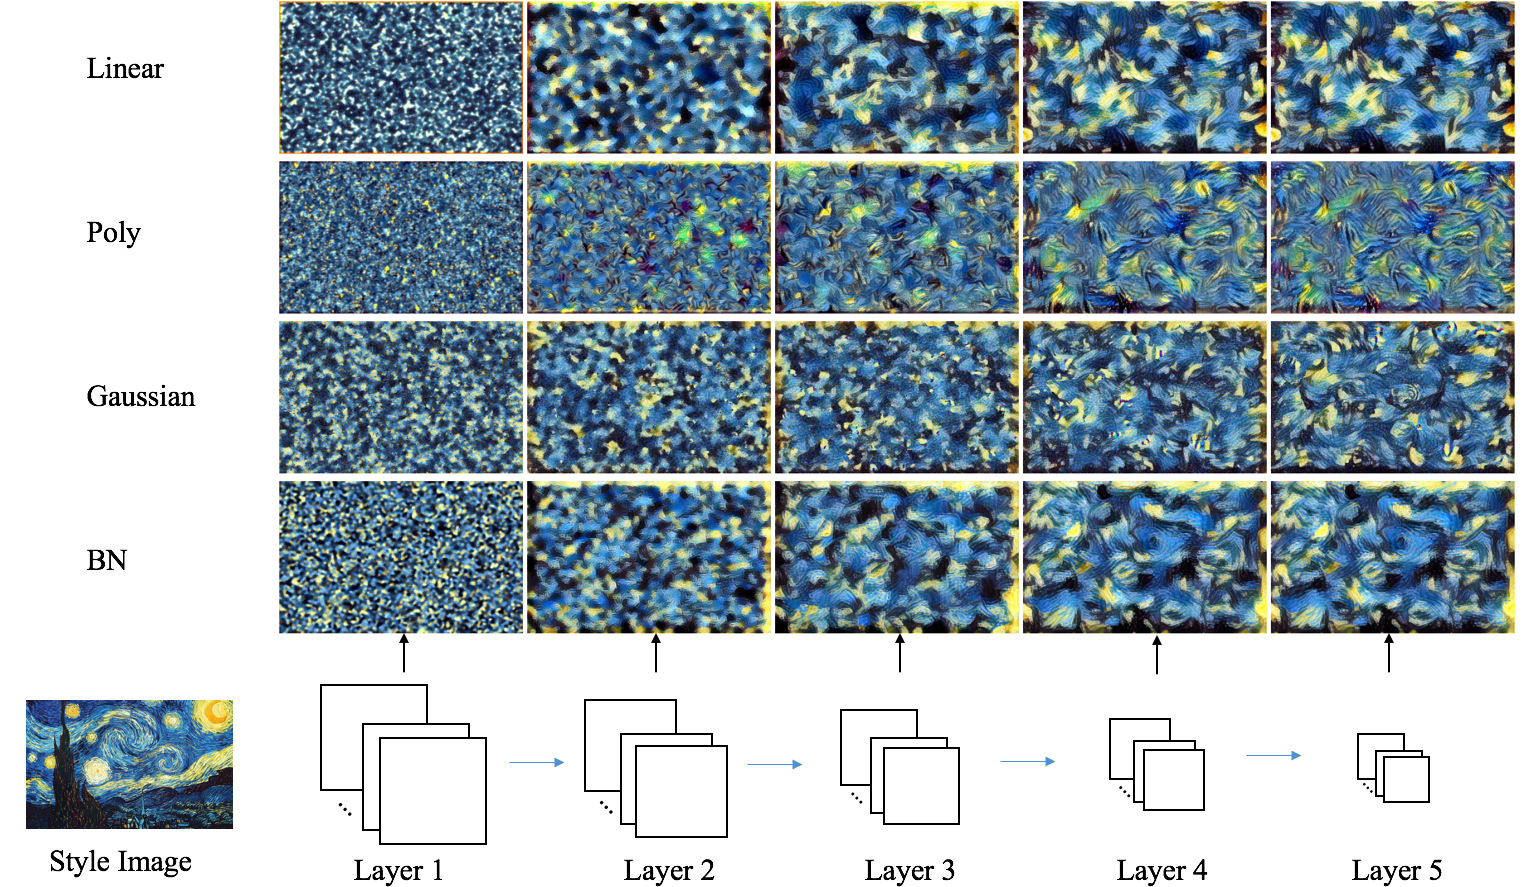
\includegraphics[width=0.98\linewidth]{style_reconstr.png}
\end{center}
\vspace{-2mm}
	\caption{Style reconstructions of different methods in five layers, respectively. Each row corresponds to one method and the reconstruction results are obtained by only using the style loss $\mathcal{L}_{style}$ with $\alpha=0$. We also reconstruct different style representations in different subsets of layers of VGG network. For example, layer 3 contains the style loss of the first 3 layers ($w_1=w_2=w_3=1.0$ and $w_4=w_5=0.0$).% The input style image is \emph{The Starry Night} by Vincent van Gogh, 1889.
	} \label{fig:style_reconstr}
\vspace{-2mm}
\end{figure}




\begin{figure*}[!htpb]
\begin{center}
	\subfigure{
	  \begin{overpic}[width=0.13\linewidth]{tubingen.jpg}%
	    \put(-5,-5){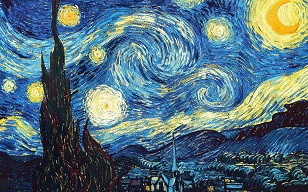
\includegraphics[width=0.08\linewidth]{starry_night.jpg}}
	  \end{overpic}
	 % \subcaption{Bicubic}
	}
	\subfigure{\includegraphics[width=0.13\linewidth]{{tubingen-starry_night-linear-0.10-1.00-m0.50}.jpg}}~~
	\subfigure{\includegraphics[width=0.13\linewidth]{{tubingen-starry_night-linear-0.20-1.00-m0.50}.jpg}}~~
	\subfigure{\includegraphics[width=0.13\linewidth]{{tubingen-starry_night-linear-1.00-1.00-m0.50}.jpg}}~~
	\subfigure{\includegraphics[width=0.13\linewidth]{{tubingen-starry_night-linear-5.00-1.00-m0.50}.jpg}}~~
	\subfigure{\includegraphics[width=0.13\linewidth]{{tubingen-starry_night-linear-10.00-1.00-m0.50}.jpg}}\\
	\vspace{-1mm}
	\subfigure{
	  \begin{overpic}[width=0.13\linewidth]{brad_pitt.jpg}%
	    \put(-5,-5){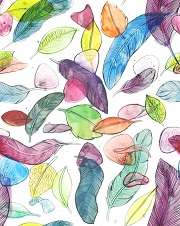
\includegraphics[width=0.08\linewidth]{feathers.jpg}}
	  \end{overpic}
	 % \subcaption{Bicubic}
	}
	\subfigure{\includegraphics[width=0.13\linewidth]{{brad_pitt-feathers-poly-c0.00-0.10-1.00-m0.50}.jpg}}~~
	\subfigure{\includegraphics[width=0.13\linewidth]{{brad_pitt-feathers-poly-c0.00-0.20-1.00-m0.50}.jpg}}~~
	\subfigure{\includegraphics[width=0.13\linewidth]{{brad_pitt-feathers-poly-c0.00-1.00-1.00-m0.50}.jpg}}~~
	\subfigure{\includegraphics[width=0.13\linewidth]{{brad_pitt-feathers-poly-c0.00-5.00-1.00-m0.50}.jpg}}~~
	\subfigure{\includegraphics[width=0.13\linewidth]{{brad_pitt-feathers-poly-c0.00-10.00-1.00-m0.50}.jpg}}\\
	\vspace{-1mm}
	\subfigure{
	  \begin{overpic}[width=0.13\linewidth]{golden_gate.jpg}%
	    \put(-5,-5){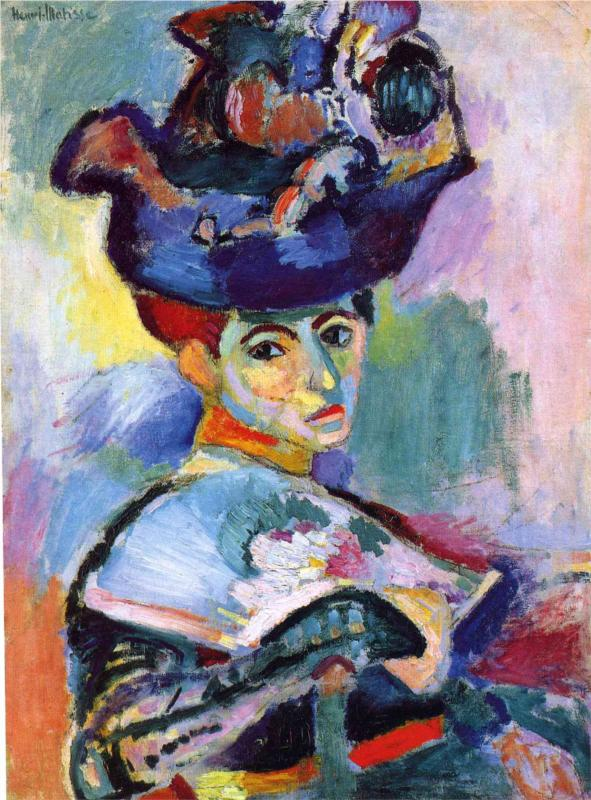
\includegraphics[width=0.05\linewidth]{woman-with-hat-matisse.jpg}}
	  \end{overpic}
	 % \subcaption{Bicubic}
	}
	\subfigure{\includegraphics[width=0.13\linewidth]{{golden_gate-woman-with-hat-matisse-gaussian-0.10-1.00-m0.50}.jpg}}~~
	\subfigure{\includegraphics[width=0.13\linewidth]{{golden_gate-woman-with-hat-matisse-gaussian-0.20-1.00-m0.50}.jpg}}~~
	\subfigure{\includegraphics[width=0.13\linewidth]{{golden_gate-woman-with-hat-matisse-gaussian-1.00-1.00-m0.50}.jpg}}~~
	\subfigure{\includegraphics[width=0.13\linewidth]{{golden_gate-woman-with-hat-matisse-gaussian-5.00-1.00-m0.50}.jpg}}~~
	\subfigure{\includegraphics[width=0.13\linewidth]{{golden_gate-woman-with-hat-matisse-gaussian-10.00-1.00-m0.50}.jpg}}\\
	\vspace{-1mm}
\setcounter{subfigure}{0}
	\subfigure[Content / Style]{
	  \begin{overpic}[width=0.13\linewidth]{hoovertowernight.jpg}%
	    \put(-5,-5){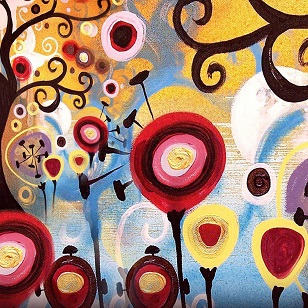
\includegraphics[width=0.05\linewidth]{candy.jpg}}
	  \end{overpic}
	 % \subcaption{Bicubic}
	}
	\subfigure[$\gamma=0.1$]{\includegraphics[width=0.13\linewidth]{{hoovertowernight-candy-bn-0.10-1.00-m0.50}.jpg}~~\label{fig:gamma0.1}}
	\subfigure[$\gamma=0.2$]{\includegraphics[width=0.13\linewidth]{{hoovertowernight-candy-bn-0.20-1.00-m0.50}.jpg}~~\label{fig:gamma0.2}}
	\subfigure[$\gamma=1.0$]{\includegraphics[width=0.13\linewidth]{{hoovertowernight-candy-bn-1.00-1.00-m0.50}.jpg}~~\label{fig:gamma1.0}}
	\subfigure[$\gamma=5.0$]{\includegraphics[width=0.13\linewidth]{{hoovertowernight-candy-bn-5.00-1.00-m0.50}.jpg}~~\label{fig:gamma5.0}}
	\subfigure[$\gamma=10.0$]{\includegraphics[width=0.13\linewidth]{{hoovertowernight-candy-bn-10.00-1.00-m0.50}.jpg}\label{fig:gamma10.0}}
\end{center}
	\caption{Results of the four methods (\emph{linear}, \emph{poly}, \emph{Gaussian} and \emph{BN}) with different balance factor $\gamma$. Larger $\gamma$ means more emphasis on the style loss.} \label{fig:effect_factor}
	\vspace{-2.5mm}
\end{figure*}


To validate that the extended neural style transfer methods can capture the style representation of an artistic image, we first visualize the style reconstruction results of different methods only using the style loss in Fig.~\ref{fig:style_reconstr}. Moreover, Fig.~\ref{fig:style_reconstr} also compares the style representations of different layers. On one hand, for a specific method (one row), the results show that different layers capture different levels of style: The textures in the top layers usually has larger granularity than those in the bottom layers. This is reasonable because each neuron in the top layers has larger receptive field and thus has the ability to capture more global textures. On the other hand, for a specific layer, Fig.~\ref{fig:style_reconstr} also demonstrates that the style captured by different methods differs. For example, in top layers, the textures captured by MMD with a linear kernel are composed by thick strokes. Contrarily, the textures captured by MMD with a polynomial kernel are more fine grained. 





\end{subsection}

\begin{subsection}{Result Comparisons}
%In this subsection, we investigate some factors that may affect the final visual results of style transfer.
\begin{paragraph}{Effect of the Balance Factor}
We first explore the effect of the balance factor between the content loss and style loss by varying the weight $\gamma$. Fig.~\ref{fig:effect_factor} shows the results of four transfer methods with various $\gamma$ from $0.1$ to $10.0$. As intended, the global color information in the style image is successfully transfered to the content image, and the results with smaller $\gamma$ preserve more content details as shown in Fig.~\ref{fig:gamma0.1} and Fig.~\ref{fig:gamma0.2}. When $\gamma$ becomes larger, more stylized textures are incorporated into the results. For example, Fig.~\ref{fig:gamma5.0} and Fig.~\ref{fig:gamma10.0} have much more similar illumination and textures with the style image, while Fig.~\ref{fig:gamma1.0} shows a balanced result between the content and style. Thus, users can make trade-off between the content and the style by varying $\gamma$.


\end{paragraph}

\begin{figure}[htpb]
\begin{center}
\subfigure{
	  \begin{overpic}[width=0.185\linewidth]{IMG_4343.jpg}%
	    \put(-5,-5){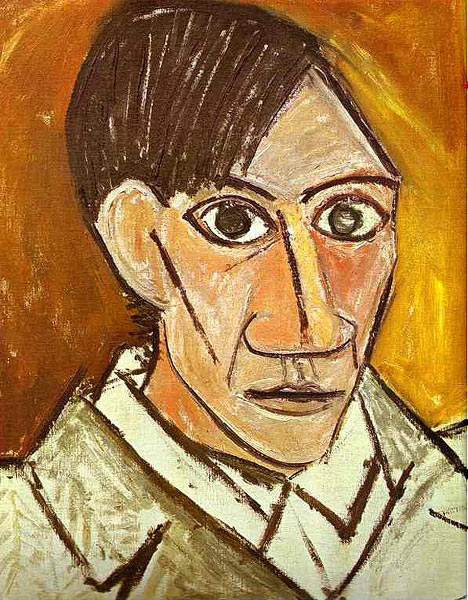
\includegraphics[width=0.08\linewidth]{picasso_selfport1907.jpg}}
	  \end{overpic}
	}
	\subfigure{\includegraphics[width=0.185\linewidth]{{IMG_4343-picasso_selfport1907-linear-2.00-1.00-m0.50}.jpg}}
	\subfigure{\includegraphics[width=0.185\linewidth]{{IMG_4343-picasso_selfport1907-poly-c0.00-2.00-1.00-m0.50}.jpg}}
	\subfigure{\includegraphics[width=0.185\linewidth]{{IMG_4343-picasso_selfport1907-gaussian-2.00-1.00-m0.50}.jpg}}
	\subfigure{\includegraphics[width=0.185\linewidth]{{IMG_4343-picasso_selfport1907-bn-2.00-1.00-m0.50}.jpg}}\\
	\vspace{-1mm}

\subfigure{
	  \begin{overpic}[width=0.185\linewidth]{golden_gate.jpg}%
	    \put(-5,-5){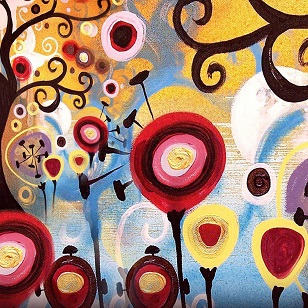
\includegraphics[width=0.08\linewidth]{candy.jpg}}
	  \end{overpic}
	}
	\subfigure{\includegraphics[width=0.185\linewidth]{{golden_gate-candy-linear-2.00-1.00-m0.50}.jpg}}
	\subfigure{\includegraphics[width=0.185\linewidth]{{golden_gate-candy-poly-c0.00-2.00-1.00-m0.50}.jpg}}
	\subfigure{\includegraphics[width=0.185\linewidth]{{golden_gate-candy-gaussian-2.00-1.00-m0.50}.jpg}}
	\subfigure{\includegraphics[width=0.185\linewidth]{{golden_gate-candy-bn-2.00-1.00-m0.50}.jpg}}\\
	\vspace{-1mm}

\subfigure{
	  \begin{overpic}[width=0.185\linewidth]{chicago.jpg}%
	    \put(-5,-5){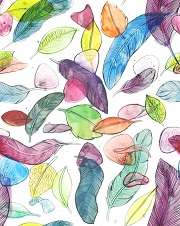
\includegraphics[width=0.08\linewidth]{feathers.jpg}}
	  \end{overpic}
	}
	\subfigure{\includegraphics[width=0.185\linewidth]{{chicago-feathers-linear-2.00-1.00-m0.50}.jpg}}
	\subfigure{\includegraphics[width=0.185\linewidth]{{chicago-feathers-poly-c0.00-2.00-1.00-m0.50}.jpg}}
	\subfigure{\includegraphics[width=0.185\linewidth]{{chicago-feathers-gaussian-2.00-1.00-m0.50}.jpg}}
	\subfigure{\includegraphics[width=0.185\linewidth]{{chicago-feathers-bn-2.00-1.00-m0.50}.jpg}}\\
	\vspace{-1mm}

\subfigure{
	  \begin{overpic}[width=0.185\linewidth]{tubingen.jpg}%
	    \put(-5,-5){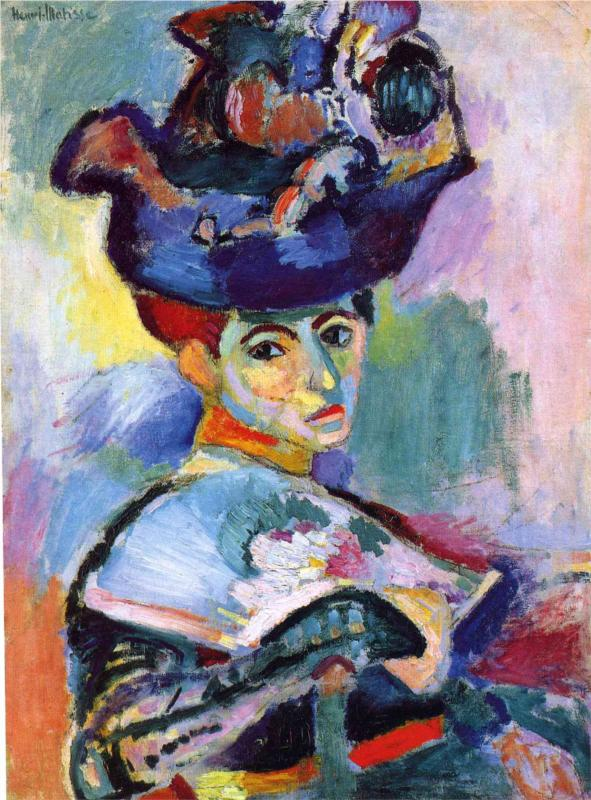
\includegraphics[width=0.08\linewidth]{woman-with-hat-matisse.jpg}}
	  \end{overpic}
	}
	\subfigure{\includegraphics[width=0.185\linewidth]{{tubingen-woman-with-hat-matisse-linear-5.00-1.00-m0.50}.jpg}}
	\subfigure{\includegraphics[width=0.185\linewidth]{{tubingen-woman-with-hat-matisse-poly-c0.00-5.00-1.00-m0.50}.jpg}}
	\subfigure{\includegraphics[width=0.185\linewidth]{{tubingen-woman-with-hat-matisse-gaussian-5.00-1.00-m0.50}.jpg}}
	\subfigure{\includegraphics[width=0.185\linewidth]{{tubingen-woman-with-hat-matisse-bn-5.00-1.00-m0.50}.jpg}}\\
	\vspace{-1mm}


\subfigure{
	  \begin{overpic}[width=0.185\linewidth]{brad_pitt.jpg}%
	    \put(-5,-5){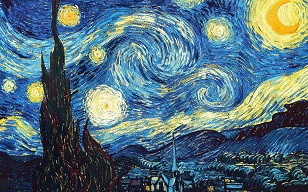
\includegraphics[width=0.08\linewidth]{starry_night.jpg}}
	  \end{overpic}
	}
	\subfigure{\includegraphics[width=0.185\linewidth]{{brad_pitt-starry_night-linear-5.00-1.00-m0.50}.jpg}}
	\subfigure{\includegraphics[width=0.185\linewidth]{{brad_pitt-starry_night-poly-c0.00-5.00-1.00-m0.50}.jpg}}
	\subfigure{\includegraphics[width=0.185\linewidth]{{brad_pitt-starry_night-gaussian-5.00-1.00-m0.50}.jpg}}
	\subfigure{\includegraphics[width=0.185\linewidth]{{brad_pitt-starry_night-bn-5.00-1.00-m0.50}.jpg}}\\
	\vspace{-1mm}

\setcounter{subfigure}{0}
\subfigure[Content / Style]{
	  \begin{overpic}[width=0.185\linewidth]{hoovertowernight.jpg}%
	    \put(-5,-5){\includegraphics[width=0.08\linewidth]{la_muse.jpg}}
	  \end{overpic}
	}
	\subfigure[linear]{\includegraphics[width=0.185\linewidth]{{hoovertowernight-la_muse-linear-5.00-1.00-m0.50}.jpg}}
	\subfigure[poly]{\includegraphics[width=0.185\linewidth]{{hoovertowernight-la_muse-poly-c0.00-5.00-1.00-m0.50}.jpg}}
	\subfigure[Gaussian]{\includegraphics[width=0.185\linewidth]{{hoovertowernight-la_muse-gaussian-5.00-1.00-m0.50}.jpg}}
	\subfigure[BN]{\includegraphics[width=0.185\linewidth]{{hoovertowernight-la_muse-bn-5.00-1.00-m0.50}.jpg}}\\
	\vspace{-1mm}

\end{center}
	\caption{Visual results of several style transfer methods, including \emph{linear}, \emph{poly}, \emph{Gaussian} and \emph{BN}. The balance factors $\gamma$ in the six examples are $2.0$, $2.0$, $2.0$, $5.0$, $5.0$ and $5.0$, respectively.} \label{fig:vis_results}
%		\vspace{-10mm}
\end{figure}


\begin{figure*}[htpb]
\begin{center}
	\subfigure{
	  \begin{overpic}[width=0.14\linewidth]{hoovertowernight.jpg}%
	    \put(-5,-5){\includegraphics[width=0.08\linewidth]{starry_night.jpg}}
	  \end{overpic}
	}
	\subfigure{\includegraphics[width=0.14\linewidth]{{hoovertowernight-starry_night-bn,poly-c0.00-5.00-1.00-m0.90}.jpg}}
	\subfigure{\includegraphics[width=0.14\linewidth]{{hoovertowernight-starry_night-bn,poly-c0.00-5.00-1.00-m0.70}.jpg}}
	\subfigure{\includegraphics[width=0.14\linewidth]{{hoovertowernight-starry_night-bn,poly-c0.00-5.00-1.00-m0.50}.jpg}}
	\subfigure{\includegraphics[width=0.14\linewidth]{{hoovertowernight-starry_night-bn,poly-c0.00-5.00-1.00-m0.30}.jpg}}
	\subfigure{\includegraphics[width=0.14\linewidth]{{hoovertowernight-starry_night-bn,poly-c0.00-5.00-1.00-m0.10}.jpg}}\\
	\vspace{-1mm}
	\subfigure{
	  \begin{overpic}[width=0.14\linewidth]{brad_pitt.jpg}%
	    \put(-5,-5){\includegraphics[width=0.08\linewidth]{candy.jpg}}
	  \end{overpic}
	}
	\subfigure{\includegraphics[width=0.14\linewidth]{{brad_pitt-candy-bn,poly-c0.00-5.00-1.00-m0.90}.jpg}}
	\subfigure{\includegraphics[width=0.14\linewidth]{{brad_pitt-candy-bn,poly-c0.00-5.00-1.00-m0.70}.jpg}}
	\subfigure{\includegraphics[width=0.14\linewidth]{{brad_pitt-candy-bn,poly-c0.00-5.00-1.00-m0.50}.jpg}}
	\subfigure{\includegraphics[width=0.14\linewidth]{{brad_pitt-candy-bn,poly-c0.00-5.00-1.00-m0.30}.jpg}}
	\subfigure{\includegraphics[width=0.14\linewidth]{{brad_pitt-candy-bn,poly-c0.00-5.00-1.00-m0.10}.jpg}}\\
	\vspace{-1mm}
	\subfigure{
	  \begin{overpic}[width=0.14\linewidth]{chicago.jpg}%
	    \put(-5,-5){\includegraphics[width=0.08\linewidth]{feathers.jpg}}
	  \end{overpic}
	 % \subcaption{Bicubic}
	}
	\subfigure{\includegraphics[width=0.14\linewidth]{{chicago-feathers-linear,gaussian-5.00-1.00-m0.90}.jpg}}
	\subfigure{\includegraphics[width=0.14\linewidth]{{chicago-feathers-linear,gaussian-5.00-1.00-m0.70}.jpg}}
	\subfigure{\includegraphics[width=0.14\linewidth]{{chicago-feathers-linear,gaussian-5.00-1.00-m0.50}.jpg}}
	\subfigure{\includegraphics[width=0.14\linewidth]{{chicago-feathers-linear,gaussian-5.00-1.00-m0.30}.jpg}}
	\subfigure{\includegraphics[width=0.14\linewidth]{{chicago-feathers-linear,gaussian-5.00-1.00-m0.10}.jpg}}\\
	%\vspace{-1mm}
\setcounter{subfigure}{0}
	\subfigure[Content / Style]{
	  \begin{overpic}[width=0.14\linewidth]{tubingen.jpg}%
	    \put(-5,-5){\includegraphics[width=0.05\linewidth]{woman-with-hat-matisse.jpg}}
	  \end{overpic}
	 % \subcaption{Bicubic}
	}
	\subfigure[(0.9, 0.1)]{\includegraphics[width=0.14\linewidth]{{tubingen-woman-with-hat-matisse-linear,gaussian-5.00-1.00-m0.90}.jpg}\label{fig:multi0.9}}
	\subfigure[(0.7, 0.3)]{\includegraphics[width=0.14\linewidth]{{tubingen-woman-with-hat-matisse-linear,gaussian-5.00-1.00-m0.70}.jpg}\label{fig:multi0.7}}
	\subfigure[(0.5, 0.5)]{\includegraphics[width=0.14\linewidth]{{tubingen-woman-with-hat-matisse-linear,gaussian-5.00-1.00-m0.50}.jpg}\label{fig:multi0.5}}
	\subfigure[(0.3, 0.7)]{\includegraphics[width=0.14\linewidth]{{tubingen-woman-with-hat-matisse-linear,gaussian-5.00-1.00-m0.30}.jpg}\label{fig:multi0.3}}
	\subfigure[(0.1, 0.9)]{\includegraphics[width=0.14\linewidth]{{tubingen-woman-with-hat-matisse-linear,gaussian-5.00-1.00-m0.10}.jpg}\label{fig:multi0.1}}
\end{center}
\vspace{-1.5mm}
	\caption{Results of two fusion methods: \emph{BN} + \emph{poly} and \emph{linear} + \emph{Gaussian}. The top two rows are the results of first fusion method and the bottom two rows correspond to the second one. Each column shows the results of a  balance weight between the two methods. $\gamma$ is set as 5.0.} \label{fig:multi}
	\vspace{-2.5mm}
\end{figure*}


\begin{paragraph}{Comparisons of Different Transfer Methods}
Fig.~\ref{fig:vis_results} presents the results of various pairs of content and style images with different transfer methods\footnote{More results can be found at\\ {{http://www.icst.pku.edu.cn/struct/Projects/mmdstyle/result-1000/show-full.html}}}. Similar to matching Gram matrices, which is equivalent to the \emph{poly} method, the other three methods can also transfer satisfied styles from the specified style images. This empirically demonstrates the correctness of our interpretation of neural style transfer: Style transfer is essentially a domain adaptation problem, which aligns the feature distributions. Particularly, when the weight on the style loss becomes higher (namely, larger $\gamma$), the differences among the four methods are getting larger. This indicates that these methods implicitly capture different aspects of style, which has also been shown in Fig.~\ref{fig:style_reconstr}. Since these methods have their unique properties, they could provide more choices for users to stylize the content image. For example, \emph{linear} achieves comparable results with other methods, yet requires lower computation complexity.




\end{paragraph}

\begin{paragraph}{Fusion of Different Neural Style Transfer Methods}
Since we have several different neural style transfer methods, we propose to combine them to produce new transfer results. Fig.~\ref{fig:multi} demonstrates the fusion results of two combinations (\emph{linear} + \emph{Gaussian} and \emph{poly} + \emph{BN}). Each row presents the results with different balance between the two methods. For example, Fig.~\ref{fig:multi0.9} in the first two rows emphasize more on \emph{BN} and Fig.~\ref{fig:multi0.1} emphasizes more on \emph{poly}. The results in the middle columns show the interpolation between these two methods. We can see that the styles of different methods are blended well using our method.




\end{paragraph}








\end{subsection}







\end{section}